%%%%%%%%%%%%%%%%%%%%%%%%%%%%%%%%%%%%%%
% LaTeX poster template
% Created by Nathaniel Johnston
% August 2009
% http://www.nathanieljohnston.com/2009/08/latex-poster-template/
%%%%%%%%%%%%%%%%%%%%%%%%%%%%%%%%%%%%%%

\documentclass[final]{beamer}
\usepackage[orientation=portrait, size=arch, scale=1.3]{beamerposter}
\usepackage{graphicx}
\usepackage[noabbrev,capitalize]{cleveref}
\usepackage{wrapfig}
\usepackage[sharp]{easylist}
\usepackage{setspace}
\DeclareGraphicsExtensions{.pdf,.png,.jpg}

\setlength{\paperwidth}{36in}
\setlength{\paperheight}{48in}
\setlength{\topmargin}{0cm}%

\newlength{\sepwid}
\newlength{\onecolwid}
\newlength{\twocolwid}
%% For three columns
\setlength{\sepwid}{0.024\paperwidth}
\setlength{\onecolwid}{0.45\paperwidth}  % (1-(3+1)*0.024)/3 = 0.30133333
\setlength{\twocolwid}{2\onecolwid}

\usetheme{confposter}
\usepackage{exscale}

\usecaptiontemplate{
\small
\structure{\insertcaptionname~\insertcaptionnumber:}
\insertcaption}

\newcommand{\newauthor}[2]{
\parbox{0.26\textwidth}{
\texorpdfstring
{
\centering
\textbf{#1} \\
\vspace{0.3\baselineskip} 
{\scriptsize \texttt{#2}}
}
{#1}
}
}
%-----------------------------------------------------------
% Name and authors of poster/paper/research
%-----------------------------------------------------------

\title{A Browser-based Neume Metadata Editor}
\author{
\vspace{0.3\baselineskip} 
\normalsize
\newauthor{Andrew Fogarty}{andrew.fogarty@mail.mcgill.ca}
\and
\newauthor{Andrew Hankinson}{andrew.hankinson@mail.mcgill.ca}
\and
\newauthor{Ichiro Fujinaga}{ich@music.mcgill.ca}
}
\institute{
\vspace{0.2\baselineskip} 
\normalsize Distributed Digital Music Archives and Libraries Lab, CIRMMT, Schulich School of Music, McGill University
}

\newcommand{\blockSpace}{\vskip 0.75ex}
%\newcommand*{\xml}[1]{\small{\texttt{<#1>}}\normalsize}
%\newcommand*{\att}[1]{\small{\texttt{@#1}}\normalsize}

%-----------------------------------------------------------
% Start the poster itself
%-----------------------------------------------------------
\begin{document}
% ensure 5cm of space at the top
\setlength{\voffset}{1 in}%

% ----------
% The Poster
% ----------
\begin{frame}[fragile,t]

\begin{columns}
\begin{column}{\onecolwid}
\begin{block}{Motivation}
The Neume Metadata Editor was developed as part of the Cantus Ultimus project [1], the goal of which is to create a graphical user interface for users to browse and search through high-quality scanned images of Medieval and Renaissance chant manuscripts using metadata and OMR technology. We wanted users to be able to construct search queries without knowing how the data is named in our database and used by the Solr [2] search engine.  To construct such an interface, we needed a system for mapping names and images onto unique neume identifiers.
%We developed the Neume Metadata Editor to satisfy these requirements.
\end{block}
%\blockSpace{}
\end{column}
\begin{column}{\onecolwid}
\begin{block}{}
\centering
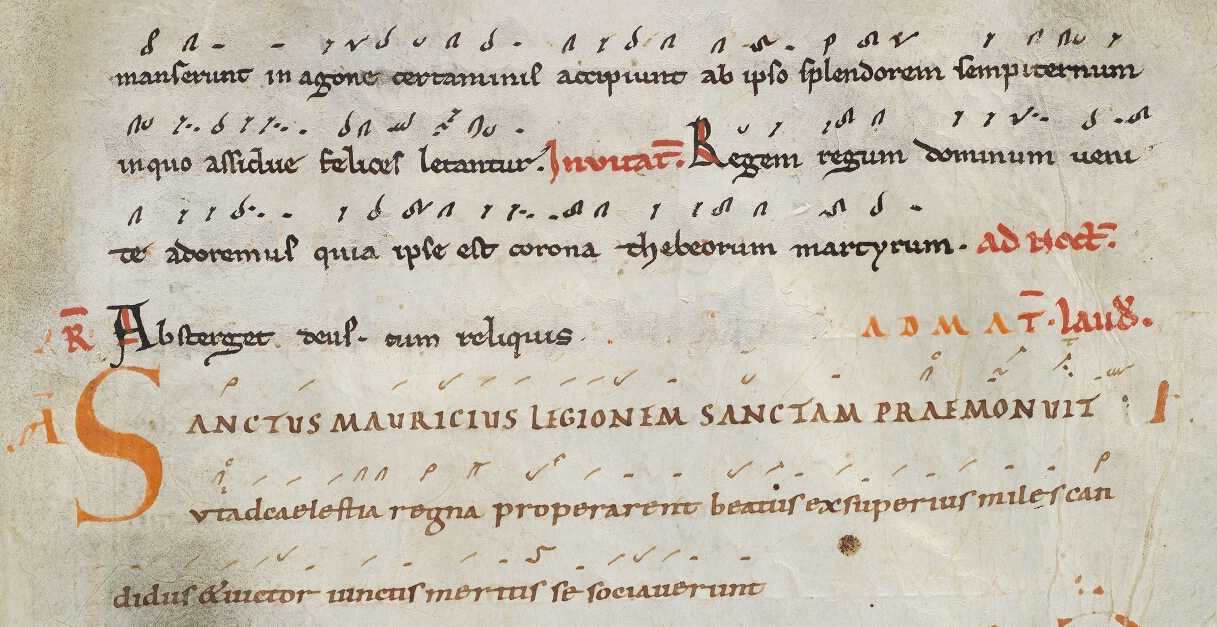
\includegraphics[width=\onecolwid]{images/different-hands.png}

%Handwriting change in the St. Gallen 391 manuscript
\end{block}
%\blockSpace{}

\end{column}
\end{columns}

%\vspace{2cm}

\begin{columns}
\begin{column}{\onecolwid}
\begin{block}{}
\centering
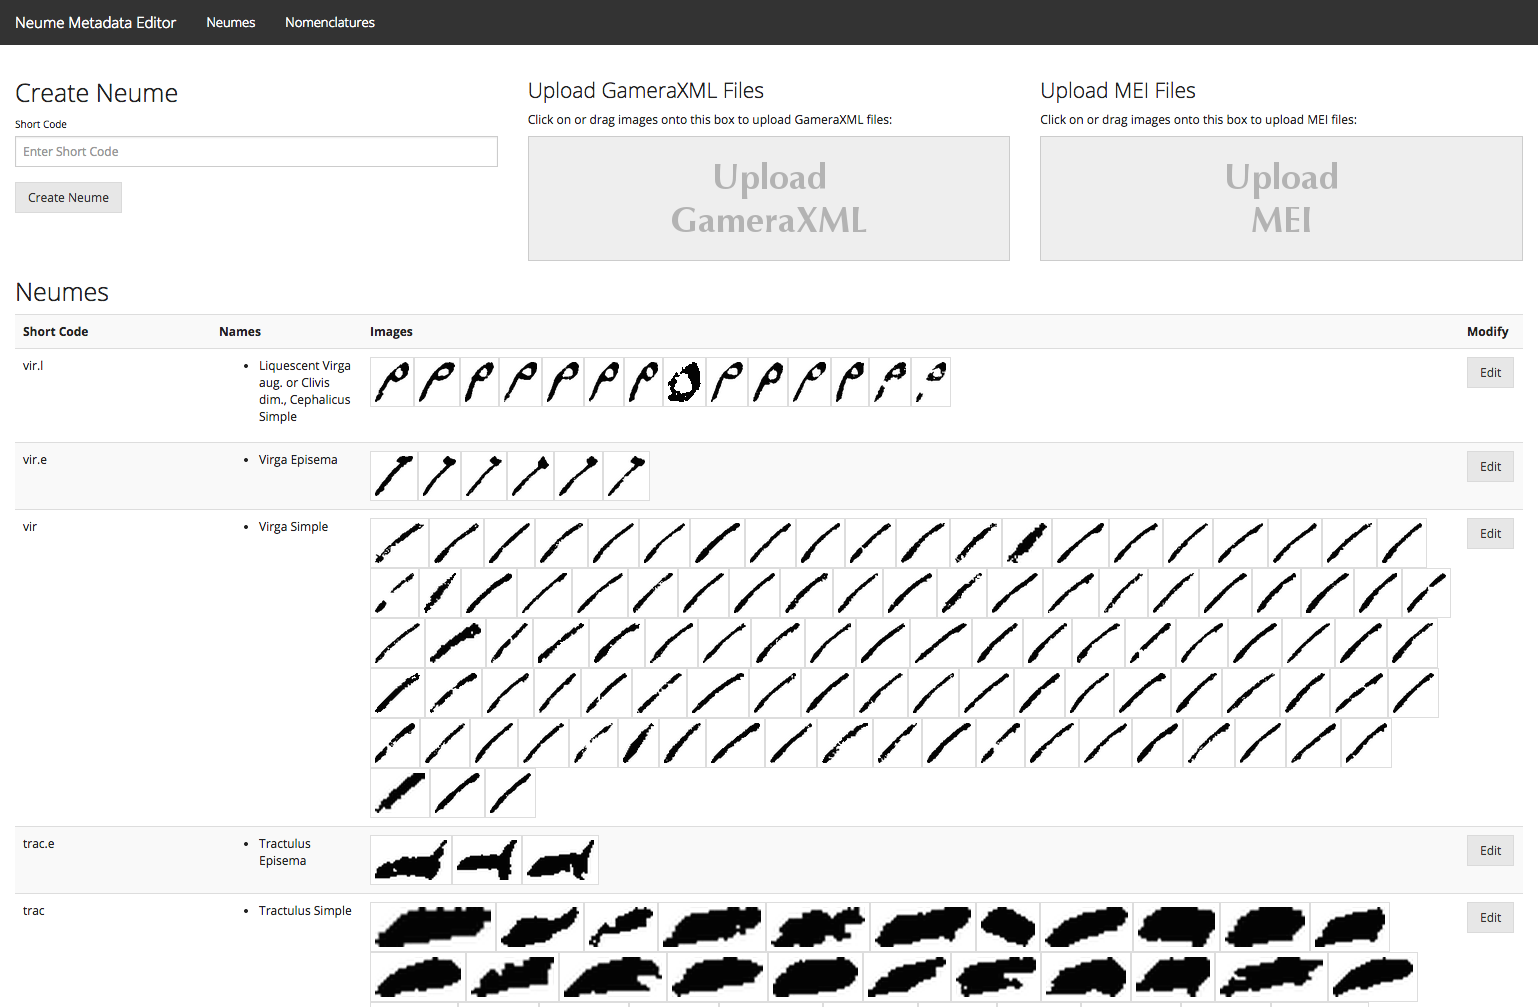
\includegraphics[width=\onecolwid]{images/neume-list-interface_cropped.png} 

The Editor, showing a list of neumes, names, and images
\end{block}
%\blockSpace{}
\end{column}

\begin{column}{\onecolwid}
\begin{block}{Design}
\begin{center}
\vspace{-0.25\baselineskip}
\small{http://github.com/DDMAL/cantus/}
\normalsize
\vspace{0.25\baselineskip}
\end{center}

\raggedright

The design goals were to:

\begin{easylist}[itemize]
%\ListProperties(Margin1=0cm, Margin2=3cm)
# Store neumes, names, and images as unique objects.
# Represent neume types with single, canonical identifiers.
# Establish neume-to-name and neume-to-image relationships.
# Distinguish between neumes of the same type and neumes of different types.
# Store images that depict the same neume type in different handwriting styles.
# Provide browser-based GUI and RESTful API.
%# Name from a set can be used to retrieve the neume identifier or the corresponding set of neume images.
%## Client applications can make these kinds of retrievals by using representational state transfer (REST) to communicate directly.
%# System avoids redundancy in how we index instances of neumes in our Cantus Ultimus search engine.
%## JavaScript search interface makes only one request to the Neume Metadata Editor and then handles the rest of the name-to-identifier translation on the client-side in real-time.
\end{easylist}

% The Neume Metadata Editor treats names and images as unique objects that exist in relation to neume types. By establishing these neume-to-name and neume-to-image relationships our system can distinguish between neumes of the same type and neumes of different types. Researchers can enter neume data manually or import neume data from MEI files.
% Once a set of names have been mapped to a neume identifier, any name from the set can be used to retrieve the neume identifier or the corresponding set of neume images.
% Client applications can make these kinds of retrievals by using representational state transfer (REST) to communicate with the Neume Metadata Editor directly.\\
%\vspace{\baselineskip}

% By using the Neume Metadata Editor to categorize neume types, we avoid redundancy in how we index instances of neumes in our Cantus Ultimus search engine. Rather than indexing multiple names for every single neume instance, we represent neume types with single, canonical identifiers. The JavaScript search interface makes only one request to the Neume Metadata Editor and then handles the rest of the name-to-identifier translation on the client-side in real-time.

%\vspace{-1.6cm}
\end{block}


%\blockSpace{}

\end{column}

\end{columns}

%\vspace{2cm}

\begin{columns}
\begin{column}{\onecolwid}
%\vspace{2.2cm}
\begin{block}{The Editor \& API}
\raggedright
Browser-based web application for editing neume metadata.  Users can:
\begin{easylist}[itemize]
%\ListProperties(Margin1=0cm, Margin2=3cm)
# Create, update, and delete neumes, names, and images.
# Assign names to unique neume identifiers.
# Group names by user-defined nomenclatures.
# Assign glyph images to unique neume identifiers.
# Upload GameraXML and MEI files to extract names and images.
\end{easylist}

RESTful API for easy integration with external client applications, which can:
\begin{easylist}[itemize]
%\ListProperties(Margin1=0cm, Margin2=3cm)
# Retrieve names and images for particular neumes and nomenclatures.
# Create, modify, and delete  neumes, names, images, and nomenclatures.
\end{easylist}
\end{block}
\end{column}

\begin{column}{\onecolwid}
\begin{block}{}
\centering
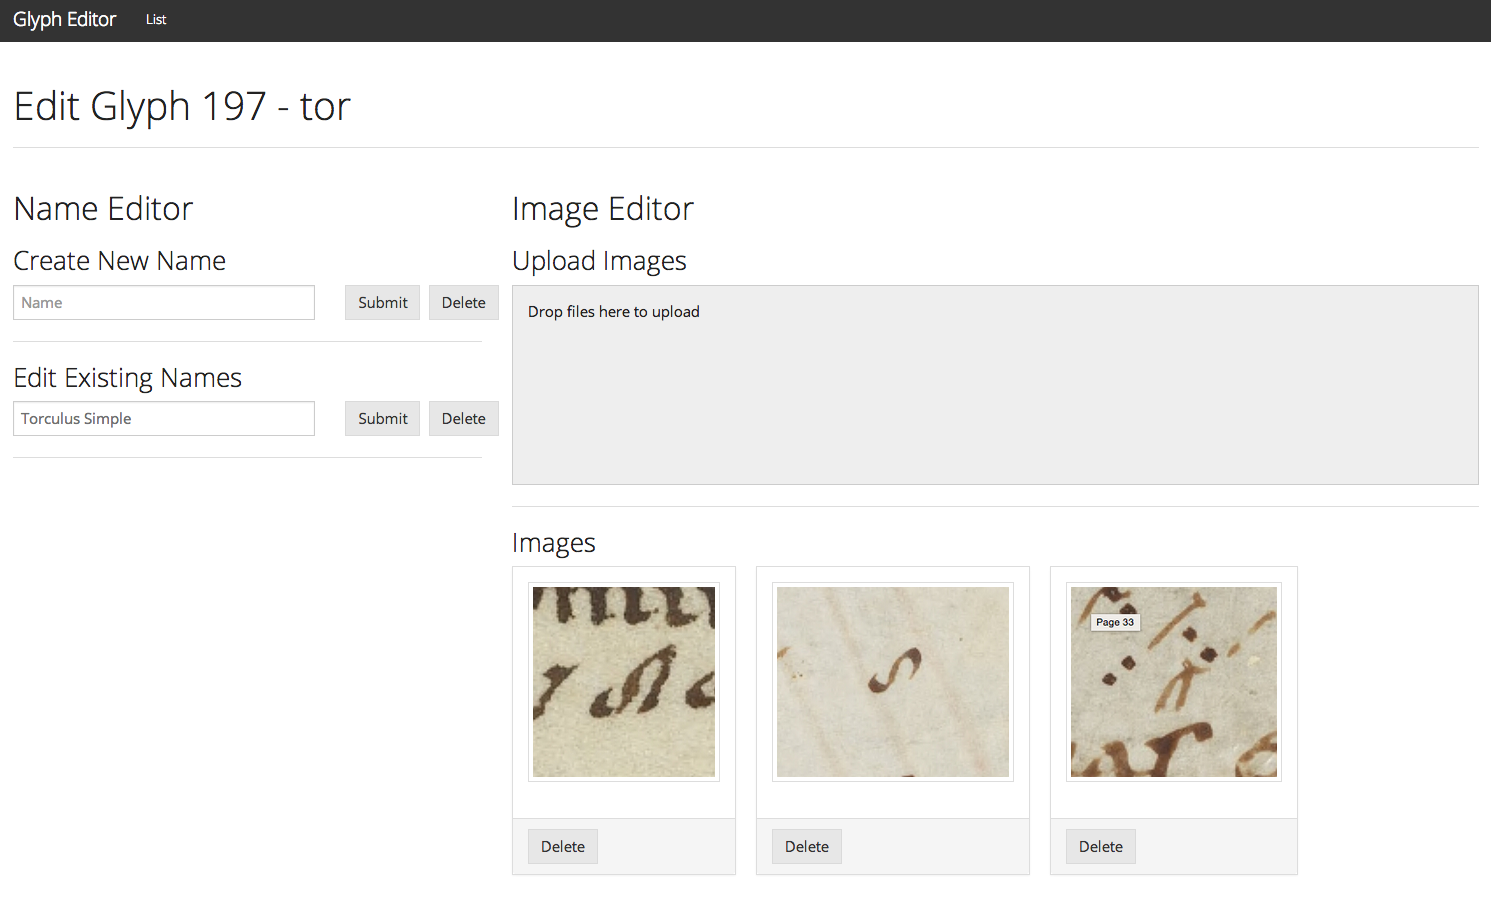
\includegraphics[width=\onecolwid]{images/web-interface.png} 

Editing a ``Virga Episema'' neume
\end{block}
%\blockSpace{}

\end{column}
\end{columns}

%\vspace{2cm}

\begin{columns}
\begin{column}{\onecolwid}
\begin{block}{References}
\footnotesize
[1] http://cantus.simssa.ca/        

[2] http://lucene.apache.org/solr/
\end{block}  
\blockSpace{} 

\begin{block}{Acknowledgements}     
This research was supported by the Social Sciences and Humanities Research Council of Canada.
\end{block}

\end{column}
\begin{column}{\onecolwid}
\begin{block}{}
\vspace{-2cm}
\centering

\includegraphics[scale=0.2625]{images/McGill_logo}
\hspace{1.2cm} 

\includegraphics[scale=0.75]{images/Schulich_logo}
\hspace{1.2cm} 

\includegraphics[scale=0.2625]{images/CIRMMT_logo}

\centering

\includegraphics[scale=0.36]{images/ddmal_logo_large}

\includegraphics[scale=1]{images/SIMSSA_logo}


\includegraphics[width=\onecolwid]{images/SSHRC_logo}
\end{block}
\end{column}
\end{columns}

\vspace{1em}

Music Encoding Conference 2015
\end{frame}

\end{document}
